\documentclass [11pt, proquest] {uwthesis}[2020/02/24]
\usepackage{graphicx}
\graphicspath{ {./images/} }

\setcounter{tocdepth}{1}  % Print the chapter and sections to the toc

\let\mffont=\sf

\begin{document}

\prelimpages

\Title{Securing WireGuard private keys with a hardware token\\}
\Author{Peter Van Eenoo}
\Year{2022}
\Program{Computer Science and Engineering}

\Chair{Brent Lagesse}{Dr.}{Computing \& Software Systems}
\Signature{William Erdly}
\Signature{Yang Peng}

\copyrightpage

\titlepage  


\setcounter{page}{-1}
\abstract{

WireGuard is a popular, secure, and relatively new VPN implementation that has seen widespread adoption. WireGuard's basic key management in the reference implementation leaves some weaknesses that could be exploited by threat actors to steal keys, compromising a user's identity or exploit their privilege. In my project I combined the industry-standard practice of isolating sensitive data with cutting-edge support for Curve25519 keys on select security keys. I created a WireGuard-compatible fork called WireGuard-HSM which uses the PKCS\#11 interface to securely store a user's private key and perform privileged operations on a USB security key. Using a comparative threat model analysis, I show how my modifications improve the security of the system by decreasing the attack surface of WireGuard. WireGuard-HSM is more immune to malware and threat actors while allowing a user to securely 'carry' their identify with them and move between machines, all without a noticeable performance penalty. 

}

\tableofcontents
\listoffigures

\chapter*{Glossary}      % starred form omits the `chapter x'
\addcontentsline{toc}{chapter}{Glossary}
\thispagestyle{plain}

\begin{glossary}

\item[WireGuard]

a VPN technology created in 2017 by Jason DonenFeld that operates at the network layer. It aims to be a replacement for popular TLS-based VPNs like OpenVPN and IPsec. WireGuard uses a fixed-set of cryptographic primitives and by design, has no support for negotiation of these primitives. 

\item[Curve25519]
an elliptic curve with a 256-bit key size. Designed by Daniel J. Bernstein in 2005\cite{bernstein_curve25519_2005}. 
Curve25519 has a digital signature algorithm named Ed25519 and a key derivation algorithm named X25519.

\item[X25519]
an algorithm that uses Curve25519 to implement Elliptic-curve Diffie–Hellman (ECDH) key exchange. This process is also known as a key derivation function (KDF). All KDF references refer specifically to X25519.

\item[AEAD]
Authenticated encryption with additional data. A class of encryption algorithms which enforce confidentiality and authenticity of data. 

\item{HKDF}
Hashed Message Authentication Code (HMAC)-based key derivation function (HKDF). RFC5869 \cite{krawczyk_hmac-based_2010}

\item[AEAD]
Authenticated encryption with additional data. A class of encryption algorithms which enforce confidentiality and authenticity of data. 

\item[ChaCha20Poly1350]
an AEAD encryption algorithm which is composed of the ChaCha20 stream cipher and Poly1305 for message authentication code (MAC)

\item[PKCS\#11] a platform-independent interface standard for interacting with cyrptographic tokens governed by the OASIS technical committee\cite{noauthor_cryptsoft_2020}.
It defines a common interface for programs to interact with security keys, also referred to as cryptographic tokens.

\item[Hardware security module]
(HSM) is adedicated, physical device that safeguards digital keys and provides limited-access to the resident keys for operations on messages such as encryption, decryption, verification and authentication. 

\item[Security Key]
a general term for a class of devices that implement a limited subset of HSM functionality. Security keys store cryptographic keys and restricts access through a limited interface. These devices typically connect to a computer or smartphone via USB or NFC and are small enough to be held on a user's key-ring.
Nitrokey Start\cite{noauthor_nitrokey_nodate} or YubiKey\cite{noauthor_discover_nodate}\cite{noauthor_u2f_nodate-1} are examples of such devices.

\end{glossary}

\textpages

\chapter {Introduction} \label{introduction}

WireGuard is a new implementation of a Virtual Private Network (VPN) proposed in 2017. It has had a successful mainstream adoption, as evidenced by its recent inclusion in many open-source operating systems\cite{donenfeld_wireguard_nodate} as well as a native Windows kernel module\cite{noauthor_wireguard-nt_nodate}. MacOS, iOS, Android, FreeBSD and OpenBSD are supported as well.
WireGuard has been described as “crypto-opinionated”, meaning the protocol supports only one cryptographic primitive for each cryptographic requirement which allows it to completely forego cryptographic-protocol negotiation between peers, eliminating design complexity and reducing it's attack surface. 

For example, WireGuard only supports Curve25519 key pairs for client authentication and key exchange, and ChaCha20Poly1350 for symmetric 
encryption\cite{donenfeld_wireguard_2017} of data.
Simplicity is a design goal of WireGuard, the protocol is implemented in under 4,000 lines of code and connection state is managed solely by the peers, no connection-state information is sent over the wire, making it difficult to track by adversaries.

WireGuard has been shown to be very fast, out-performing IPsec and OpenVPN-based VPNs, in terms of throughput and response time\cite{donenfeld_performance_2018}, as well as easy to quickly port to a wide variety of operating systems. 

An important design simplification of WireGuard is the management of public and private keys. WireGuard does not use traditional x509 digital certificates or public key infrastructure. A peer's identity is anchored to a static Curve25519-based public key stored in the plain-text configuration file.
The static public keys of the initiator and responder must be pre-shared with both parties respectively, before a successful handshake can be made. 
Proper key management is left up to system administrators however this exposes a weakness in reference implementation of WireGuard as this presents an attractive target for threat actors.

These design choices are not without their significant downsides. The lack of cryptographic negotiation means that if vulnerabilities are identified and a cryptographic component must be modified or replaced, this will result in complete peer incompatibility, until all peers are updated to the new protocol. This also means that project forks are limited in the scope of changes they can introduce, if they wish to maintain interoperability with mainline WireGuard peers.

HSM are widely used, industry-standard devices that are used to safeguard digital keys. Many HSM undergo rigorous testing and certification, to validate their compliance  with internationally recognized standards with as FIPS (TODO CITE ).

In order to address the problem of WireGuard's weak local-key management, while maintaining compatibility with mainline clients, I created a project called WireGuard-HSM. The primary design of WireGuard-HSM moves the client's private key onto a USB-security key with cutting-edge support for Curve25519 all while maintaining compatibility with mainline WireGuard clients. 

\subsection{Problem Definition} \label{problem_definition}
Since it's introduction in 2017, the WireGuard protocol has been shown to secure in many scenarios. However, after examining the reference implementation, WireGuard's management of private keys was shown to be an area for improvement. Another team of researchers have identified this weakness and we will briefly discuss their approach in section \ref{related_work}.

\subsection{Goals}
In this project, my primary goal is to increase the security of WireGuard by improving it's key handling. I want to use well established methods in the computer security field to achieve this goal, without sacrificing compatibility. Instead of proposing compatibility-breaking changes, my secondary goal was to work within the confines of the existing protocol and maintain client compatibility, while improving security. I also wanted to understand what performance implications my design choices would impose on the system. System performance is discussed in section \ref{performance}

\subsection{Outline}
I will discuss the WireGuard handshake process in enough detail so readers can understand why my changes are relevant.
I will show how weaknesses in WireGuard's key management could lead to a threat actor compromising a private key and thereby a user's identity. 
I will briefly discuss what happens to the WireGuard system when a user's identify is compromised and why a threat actor might want to do this.
I will show how the security architecture design WireGuard-HSM safeguards a user's identity in the same scenarios.
Finally I will evaluate any performance impact of WireGuard-HSM on the system and the implications for usability.



\section {Contributions}
The Elliptic Curve, Curve25519 is being used in an increasing number of open-source and commercial products from SSH to Signal\cite{noauthor_things_2022}, however hardware support in 
security keys is currently almost non-existent. YubiKey is currently the most popular security key manufacturer however all of their current products 
lack support for X25519. One of the goals of this project, as the first open source project to combine an X25519 supported security key with a popular open source VPN like WireGuard, will encourage more manufactures to add support for X25519 across the security key industry.

\chapter {Related-work}
\label{related_work}
The WireGuard handshake protocol has gone through extensive formal verification using Tamarin proof system \cite{donenfeld_formal_2018}. Researchers have identified some potential weaknesses in WireGuard around quantum computers\cite{hulsing_post-quantum_2021} but no serious vulnerabilities have been identified, since it was introduced five years ago in 2017.

WireGuard's key handling is a current area of research. A paper by \cite{wu_sewg_2020} focused on modifying WireGuard to use Trusted Execution Environment (TEE) of an Android phone to securely store the long-term static private key. The TEE is similar to the secure enclave in Intel processors. This work has the benefit that is supports a mobile operating system but it's implementation is restricted to a specific android maker's platform.

\section {Project scope}

My project is focused on improving WireGuard's handling of its private key.
It will be necessary to understand importance of the private key and how it's used during the WireGuard handshake process, when we discuss our threat model in section \ref{wg-ref-analysis}. Next I will key components of my project WireGuard-HSM.


\chapter {Background}
12)  2.1 -- Background is more about "what does the reader need to know that I don't expect somebody with a BS or MS in CS to know". Here you should be describing details about curve25519, Nitrokey, pkclient, GnuPG, etc that are relevant to why you did your work the way you did. (Conception)
\section {WireGuard Background}  \label{background}
WireGuard makes exclusive use of Curve25519 for user authentication and authorization. I will discuss it's technical use in WireGuard as well as how it is used for user identity. My project is directly involved with WireGuard's handshake process so I will provide a detailed description of it's process-flow so readers can understand the context of my projects modifications.

\subsection{Curve25519 key pairs} \label{x25519}
Curve25519 is a patent-free, high-performance elliptic-curve with a reference implementation that is in the public-domain. This makes it an attractive curve for many projects \cite{noauthor_things_2022}.
A useful feature of Curve25519 is that any 32-byte value is a valid private key. Meaning no Curve25519 key requires validation which helps avoid small subgroup attacks. Curve25519 keys have also been shown to be immune to some classes of timing attacks\cite{noauthor_safecurves_2022}\cite{sasdrich_implementing_2015}.  Deriving the public key from the private key is fast enough that programs such as WireGuard don't need to store the client's public key in their configuration file. WireGuard only saves the private key and simply derives the public key on program start-up.

WireGuard makes exclusive use of Curve25519 for peer authentication and authorization. A user's identity is rooted in their Curve25519 'long-term static public key' which is generated from their private key and shared out-out-band with every peer a users needs to communicate with. 
This public key never expires and there are no mechanisms for key revocation built into the WireGuard protocol. it doesn't expire and is the cornerstone for a user's identity. 

WireGuard also creates short-lived Curve25519 key pairs which are independent of the long-term static public key. These short-lived key pairs are referred to as the ephemeral session keys and they used to securely send the symmetric key to a peer during the handshake. Another important point is that these ephemeral session key-pairs are only valid for a default of 2 minutes per session. WireGuard has a novel key rotation mechanism which guarantees that nonce-reuse never happens but further discussion of this is out-of-scope for this paper. 

\subsection {Identity and Handshake Initiation}

\subsubsection{Handshake Initiation}
\label{sec:handshakeInitiation}
WireGuard assumes that each party's public key is securely exchanged out-of-band. This exchange must take place before a handshake can be performed. WireGuard refers to parties as an initiator and a responder, since there is no strict definition of client or server. A handshake is performed using an initiation message, sent by the initiator to the responder. 

This handshake has been described as a 1.5 round-trip-time (RTT) handshake over UDP which is inherently connection-less. The 1.5 RTT handshake is defined by the following steps: the initiator sends a handshake initiation message, the peer responds to a properly authenticated initiation message with a handshake response message. Finally the initiator sends the first data packet. These three message are required for the session to be considered established and compose the 1.5 RTT handshake process. Consider the similarity to TCP's three-way-handshake.

\begin{figure}[ht]
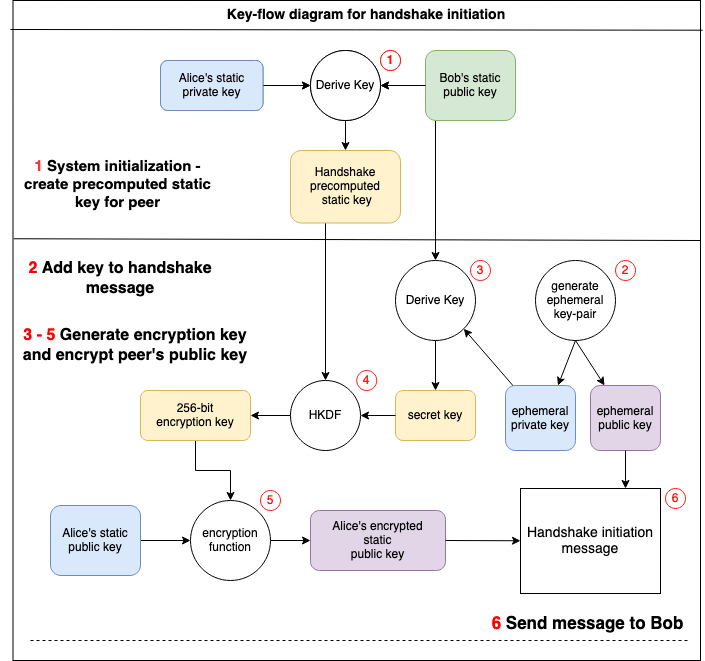
\includegraphics[width=15cm]{paper/images/key-flow-wg.drawio.png}
\caption{Detailed Handshake Initiation Process}
\label{fig:keyflow}
\end{figure}

Let's call the initiator Alice and the peer (the responder) Bob.
The diagram in \ref{fig:keyflow} shows the detailed process on Alice's computer that WireGuard goes through to send a handshake initiation message. First, WireGuard reads Alice's private key and Bob's public key from it's configuration file, sending them to a KDF to generate the handshake's precomputed-static key. Second, Alice generates an ephemeral Curve25519 key-pair and attaches that public key to her initiation message. The ephemeral private key and the precomputed static key from step 1, are used as input to an HKDF which generates, what WireGuard refers to as the chaining key. This chaining key is the key that Alice will use for symmetric encryption of her data that she will send to Bob. (TODO Confirm) The chaining key is also used as the key for ChaCha2020 encryption function which also takes Alice's static public key as input. The encrypted form of Alice's public key is finally added to the handshake initiation message.

When Bob receives this message, assuming he already has Alice's public key, he will follow this process in reverse-order. Bob will generate his own ephemeral key-pair and send the ephemeral public key in his handshake response message to Alice. The state is now identical for both peers and they each know the symmetric encryption key to decrypt data sent by the peer. It's worth noting that unlike many encryption schemes, the key to the symmetric cipher is not same in each direction because each peer chooses their own 'sending channel' cipher-key.
\subsubsection{Key Rotation}
\label{keyrotate}
WireGuard sessions guarantee perfect forward secrecy by including a key rotation process (rekey) between peers. This rekey event occurs after a default of 120 seconds, or after 2\textsuperscript{60} messages have been exchanged. The key rotation process is essentially another handshake process with one key difference: if Alice is the peer performing the rekey process, then in step 1, see figure \ref{fig:keyflow}, Bob's most recent ephemeral public key is used as input to the KDF instead of his static public key. This has implications for my project which we will discuss in section \ref{pk_design}

The WireGuard protocol has no distinction between authentication and authorization. If a peer can successfully authenticate a handshake initiation message and response, then the user is allowed to freely communicate over the session, with whatever resources may be gated on or behind the WireGuard peer.
Now that we understand the handshake initiation process and session key rotation in more detail, it should be clear how the static private and public key, form the basis for a user's identity in WireGuard. We have also discussed how a user's identify is tied to authentication and authorization in WireGuard.

\begin{figure}[ht]
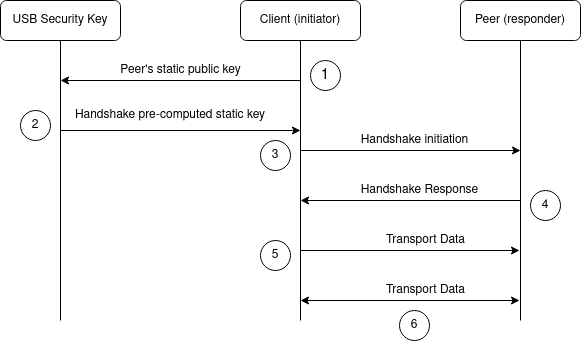
\includegraphics[width=6cm]{paper/images/Process_Diagram.drawio.png}
\caption{Informal Handshake Narration Process}
\label{fig:handshake_process}
\end{figure}

\subsection {Identity and Portability}
\label{identity}

\begin{figure}[ht]
\frame{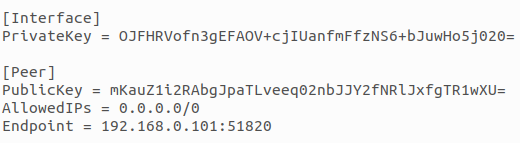
\includegraphics[width=12cm]{paper/images/wg_config.png}}
\caption{Example WireGuard Configuration File from the Reference Implementation}
\label{fig:wg_config}
\end{figure}

\subsection{Key Storage}
As mentioned previously, WireGuard leaves key management up to the user.
Figure \ref{fig:wg_config} shows an example configuration file for WireGuard. The user's private, long-term static private key is under the "[Interface]" section and "[Peer]" section contains each peer's pre-shared static public key, as well as internet address information.

WireGuard saves a user's private key as BASE64 encoded plain-text in the configuration file. There is no support for adding a password to a private key or support for traditional digital certificates. Even Curve25519 keys generated by OpenSSL are not compatible with WireGuard, unless the ANS.1 header is stripped from it's output.
If a user wants to carry their WireGuard identify with them and connect to the same peers from different machines, then the user must manage copying and securely transporting their configuration file, copying that private key into each machine's WireGuard configuration file manually. 


Here we discuss key parts of the project architecture, so readers can understand the context of the different systems that were created for this project to work.
\section{Project Design}

\begin{figure}[ht]
\begin{center}
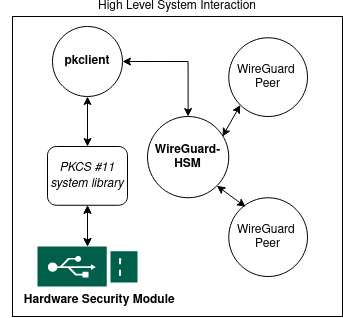
\includegraphics[width=8cm]{paper/images/high-level-overview.png}
\caption{High-Level System Interaction Diagram}
\label{fig:highlevel_system}
\end{center}
\end{figure}

Figure \ref{fig:highlevel_system} shows a high-level abstraction of the major WireGuard-HSM components. When WireGuard-HSM attempts to establish a new session with a peer, WireGuard-HSM interacts with pkclient which uses the PKCS\#11 interface to interface with a hardware security module over USB. 

\subsection{Nitrokey - Hardware Security Module}

At the time of writing, the only commercially available HSM that offered the right features features for the project was the "Nitrokey Start" from Nitrokey in Germany\cite{noauthor_nitrokey_2022}. A few HSM list support for 'Curve25519' yet most only support Ed25519 while WireGuard only uses the X25519 algorithm of Curve25519.

The Nitrokey Start connects to the computer via a USB-A interface. It securely stores cryptographic keys and provides a restricted interface based on the PKCS\#11 standard.
The HSM safeguards private keys by only allowing authenticated users to perform a strict set of key management and cryptographic function on a slot. A slot holds private and public keys and is protected by a user pin. An HSM is also designed in such a way that physical tamping with the device should render the private-keys unreadable and useless. 

\subsection{Pkclient}
\label{pk_design}
I created a standalone project called 'pkclient' to handle the interactions with the HSM and manage state. Pkclient implements functions specific to the cryptographic operations required by WireGuard but it's implemented as a standalone module to limit the required modifications to WireGuard. Pkclient itself incorporates a golang package to integrate the low-level PKCS\#11 interface calls, exposing a simplified interface to callers.  Pkclient handles the HSM session establishment, verification that the correct key-types are present on the HSM, user-interactions for pin authentication. 
From WireGuard-HSM's point of view, pkclient is responsible for key derivation functions when the long-term static private key is needed as input, which is performed inside the HSM. When the peer session expires and performs the key rotation, described in section \ref{keyrotate}, the ephemeral public key of the peer is sent in a call to pkclient to derive the new session's shared secret. 

Normally WireGuard has full-access to the long-term static private key for deriving the long-term static public key, so pkclient must also provide a function to return the public key contents, which enables the user to share their public key with other peers.


\subsection{WireGuard-HSM}
WireGuard-HSM was designed to work in a two modes, the HSM mode and the original software mode. The HSM mode has the long-term private static key completely absent, replaced by a system library path to a PKCS\#11 library and the slot number on the HSM to use, see an example file in section \ref{fig:wg_hsm_config}. The software mode is the original, unchanged mode that has access to the private key in the configuration file. WireGuard-HSM executes it's program flow in the same way as WireGuard-go but it used if/else statements to access the HSM or software mode. Having both modes allowed me to verify that the protocol was not changed in any way so I don't introduce new security vulnerabilities. In places where WireGuard expects access to the private key, changes were made to use the interface with pkclient for those calls instead. This approach helped me ensure that no incompatibility was introduced into the system. 

Simplicity and separation of privileges were primary goals in my system design so by design WireGuard-HSM abstracts much of it's functionality over to pkclient, keeping the changes to the WireGuard-go code-base to a minimum. 

Some small changes were made to the wireguard-tools package to allow configuration file changes for WireGuard-HSM to work but they out of scope for our purposes and only affect program initialization.

\begin{figure}[ht]
\frame{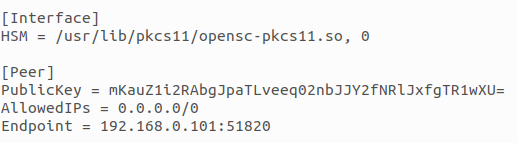
\includegraphics[width=12cm]{paper/images/wg-hsm_config.png}}
\caption{Example WireGuard-HSM Configuration File}
\label{fig:wg_hsm_config}
\end{figure}

\chapter {Methodology}
TODO WORK ON THIS
Threat modeling WireGuard's key handling initially identified weaknesses  which informed the design of WireGuard-HSM. We will discuss that threat model in section \ref{wg-ref-analysis}.
The secrecy of a client's private key is paramount to proper client authentication and authorization in WireGuard. WireGuard's design protects many aspects of the key handling that have been error prone in past VPN designs (TODO )
My threat model is based around the secrecy of the private key and reducing the risk found in the reference implementation of WireGuard. Since WireGuard allows clients protected-access to resources across networks, there is value for an attacker to gain access. 
There are two main threats to this privacy. Malware infecting a computer running the reference implementation of WireGuard. The malware could be resident on the computer or it could be a single instance where a browser exploit allows an arbitrary file to be read. Our guards against malware that runs on user's computer and gains access to the plain-text configuration file for WireGuard, leaking the private key which gives the bad-actors the ability to connect to the configured wireguard-peers undetected, as the legitimate user.


===this is where you describe the design of your system and justify your design choices.  Typically this chapter would also include any relevant models that you're using such as the threat model, user model, system model, etc. along with your design goals so that the reader knows exactly what problems you're trying to address and which ones are out of scope.===

In the following section, I discuss the threat models for WireGuard and WireGuard-HSM, comparing WireGuard-HSM to see the relative strengths and weaknesses. This will help evaluate the system design perform a comparative threat model analysis of the reference implementation and WireGuard-HSM. This analysis will show the relative strengths and weaknesses of the designs and what I have improved on.

I will also use some traditional software metrics to evaluate the project.


\section{Compatibility}
Compatibility is an important area of consideration when modifying WireGuard. Since WireGuard has no negotiation of cryptographic primitives, any project that modifies the underlying cryptographic functions or protocol, will introduce client incompatibility, leaving the modified peers only able to communicate with peers of the same type. I designed WireGuard-HSM with this in mind, to allow WireGuard-HSM peers the ability to communicate with unmodified peers.

\chapter {Evaluation}
In order to assess the security of the system I have designed. I used various threat modeling techniques to diagram the system, create attack trees and rank threats by the simple and well-established DREAD framework. Rankings and descriptions for vulnerabilities are taken from OpenStack Security Group's use of the DREAD model\cite{noauthor_securityossa-metrics_2022}. 

DREAD scores criticized as subjective however their ranking can help us identify the relative weaknesses and priorities when addressing our system design. The scores are based on a ranking of 1-10, low to high for each category, added together and divided by the number of categories to give a final score. 
First we will discuss the threats inherent in the WireGuard reference implementation and then we will discuss the same threats with WireGuard-HSM and see if our system design improves the system security at .
\section{Threat models analysis}

\subsection {WireGuard - Reference Implementation}
\label{wg-ref-analysis}
This threat model is focused on WireGuard's asset handling related to the private key, the security controls around it and the threat actors that could be lurking on the system. The computer running WireGuard will be considered Alice's computer and the WireGuard peer that Alice connects to is Bob. Both computers are turned on and connected to the network but Alice has not yet established a WireGuard session to Bob's computer. Refer back to section \ref{fig:handshake_process} on how WireGuard establishes a session with a peer. 

\begin{figure}[ht]
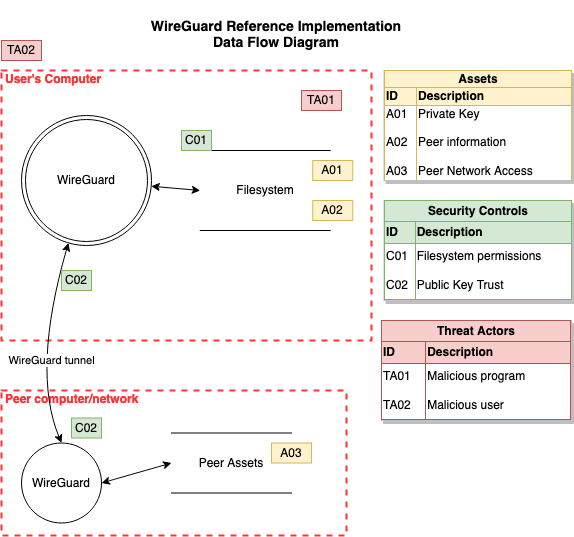
\includegraphics[width=14cm]{paper/images/WGH_DFD.drawio.png}
\caption{Threat Model for the WireGuard Reference Implementation - Data Flow Diagram}
\label{fig:wg_ref_dfd}
\end{figure}

\subsection{Assets}
The file system on Alice's computer contains the WireGuard configuration file \ref{fig:wg_config}. 
Asset A01 is Alice's Curve25519-based long-term static private key. Asset A02 is Bob's connection information consisting of his static public key and internet address. It is important to note that in this threat model, both of these assets reside in the same location. 
Asset 03 is the label for any potential assets on Bob's side of the WireGuard tunnel. Access to Bob's machine might be a highly valuable asset or Bob's network access might be the highly valuable asset. This model combines these possibilities into 'Peer Assets' for simplification.

\subsection{Security controls}
Access control in WireGuard's reference implementation for A01 and A02 is C01: file system permissions. Most of the documentation indicates that sufficient file-system permissions' should be set on the WireGuard configuration file to allow only administrator access and restrict access by unprivileged users. This is not an enforced measure, meaning WireGuard will still start and not complain if the configuration file permissions are insufficient. 

Access control C02, access to each WireGuard peer, is the public key trust system implemented by WireGuard and discussed in section \ref{sec:handshakeInitiation}.

\section{Threat Actor 1}
The primary threat is TA01: a piece of malware that has gained access to Alice's computer and will search for keys in configuration files. This malware could have been delivered by acquiring a zero-day exploit or by using a known vulnerability with a piece of software running on Alice's computer. Using a known vulnerability would likely lower the cost of the attack.


\subsection{Insufficient permissions}
If TA01 gains access to Alice's computer and the file system permissions were not correctly set on the WireGuard configuration file, then the malware gains access to A01 and A02. Access to these assets results in loss of A03 by bypassing C02. See section \ref{impersonation} to see how this works. 
ATTACK 1, ATTACK 3

\subsection{Sufficient permissions}
If C01 is configured properly, then TA01 will need exploit one more vulnerability, in-order to gain access to A01 and A02. This offers a single layer of security so the cost of this attack cost is slightly higher. Exploit chains are common-place in today's attacks so this is a reasonable assumption.  ATTACK 2, ATTACK 4

\section{Threat Actor 2}
TA02 is a malicious user who gains direct or indirect access to Alice's computer.  

In a direct method of attack, TA02 gains physical access to Alice's laptop and uses some technical or non-technical exploit to read the hard-drive. If Alice's machine uses disk-encryption then this increases the difficulty of the exploit because a second exploit must be used to read the disk contents.
ATTACK 5 and 6

The indirect method of attack could be performed by TA02 using social engineering tactics such as a phone-call or email, masquerading as someone from Alice's IT department, asking her to, in some way, disclose the contents of the WireGuard configuration file, leading to disclosure of assets A01 and A02.
ATTACK 7

\section{Vulnerabilities}
Once any of the previously weaknesses and have been taken advantage of by a threat, and the threat actor gains access to assets A01 and A02, this creates two classes of vulnerabilities in our WireGuard system.

\subsection{Impersonation}
\label{impersonation}
Loss of A01 and A02 together allow an attacker to spoof Alice's identity because the attacker can complete a handshake with Bob as Alice. VPN's are commonly used as the first layer of defense for network access, so A03 is very attractive.
This threatens confidentiality in our system between because unauthorized parties can now masquerade as authorized users. 

\subsection{Denial-of-Service}
\label{dos}
A Denial of Service vulnerability is also possible with the loss of A01 and A02. Once a threat can perform impersonation of Alice, then a DoS can be performed against Alice's WireGuard connection to Bob. When Bob receives and establishes a handshake with Alice's credentials, the initiator established that handshake with a 'sender's index'. This index is a randomly generated 4-byte value which the peer uses to identify the sessions. Once Bob has an established session with Alice's credentials, it will drop any handshake initiations messages that don't contain that index value. In this situation the attacker simply needs to establish a connection before the real Alice does, and Alice will be unable to perform a handshake with Bob until the attacker disconnects.

This denial of service attack would not be noticed by Bob because his WireGuard process already has a session established with Alice and will silently drop other connection attempts. Alice would only notice that she is unable to establish a session with Bob. Alice would have to communicate with Bob via alternative means, and have him look at his computer's WireGuard session output, then they would need to note that Alice's session is currently established and what remote IP has established the session.

A DoS attack threatens availability in the system because Alice's connection to Bob's resources can be denied by a malicious third-party.

\section{WireGuard-HSM Threat model Analysis}
\label{wg-hsm-analysis}
This threat model is also focused on WireGuard-HSM's asset handling related to the private key and peer public keys. All assumptions laid out for the previous threat model in section \ref{wg-ref-analysis} are the same here.

\begin{figure}[ht]
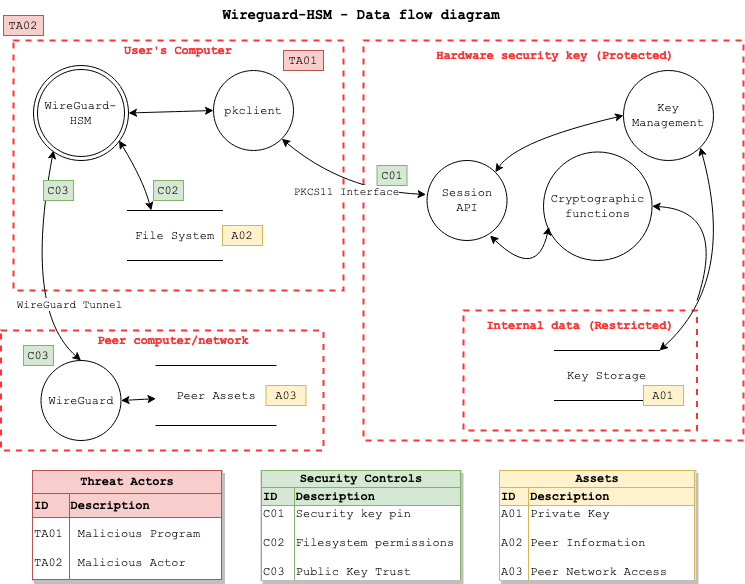
\includegraphics[width=14cm]{paper/images/WGHSM_DFD.drawio.png}
\caption{A Threat Model for WireGuard-HSM - Data Flow Diagram}
\label{fig:wg_hsm_dfd}
\end{figure}

\subsection{Assets}
The file system on Alice's computer contains the WireGuard-HSM configuration file, example in figure \ref{fig:wg_config}. 
Asset A01 is Alice's Curve25519-based long-term static private key. Asset A02 is Bob's connection information consisting of his static public key and internet address.
Asset 03 is the label for any potential assets on Bob's side of the WireGuard tunnel. Access to Bob's machine might be a highly valuable asset or Bob's network access might be the highly valuable asset. This model combines these possibilities into 'Peer Assets' for simplification.

\subsection{Security controls}
Access to asset A01 is now behind two layers of defense. Firstly A01 is now on a physically separate system, the hardware security key. Alice must plug in the HSM and authenticate with a PIN, Control C01, before cryptographic operations can be performed on A01 via the PKCS\#11 interface with the session API.
File system permissions are used to protect the Peer Information, A02.
Security control C03, access to each WireGuard peer, is the public key trust system implemented by WireGuard. See section \ref{sec:handshakeInitiation} for more detail.

\subsection{Threat Actor 1}
The primary threat is TA01: a piece of malware that has gained access to Alice's computer and will search for keys in configuration files. This malware could have been delivered by acquiring a zero-day exploit or by using a known vulnerability with a piece of software running on Alice's computer. Using a known vulnerability would likely lower the cost of the attack.

\subsubsection{Insufficient permissions}
If TA01 gains access to Alice's computer and the file system permissions were not correctly set on the WireGuard configuration file, then the threat gains access to the A02: Peer Information. Exposing the public key of a peer may be desirable but there is no direct effect or vulnerability to exploit.
ATTACK 1 and ATTACK 3

\subsubsection{Sufficient permissions}
If C01: File system permissions, is configured properly, then TA01 will have a difficult time gaining access to A02. This offers a single layer of security, so TA01 will need to perform a pivot in order to bypass the file system permissions. Performing a pivot and gaining access to A02 at this point is less lucrative because A01: Alice's private key is still not accessible to the attacker on this system.
ATTACK 2, ATTACK 4

\subsection{Threat Actor 2}
TA02 is a malicious user who gains direct or indirect access to Alice's computer. 

\subsubsection{Physical Access}
In a direct method of attack, TA02 gains physical access to Alice's laptop and uses some technical or non-technical exploit to read the hard-drive. If Alice's machine uses disk-encryption then this increases the difficulty of the exploit because a second exploit must be used to read the disk contents.
This will only result in loss A02: Peer Information but A01 is held on Alice's security key which is safely kept on her person.
ATTACK 5 and 6 

If Alice left her security key permanently connected to her computer, then there is a risk that the threat actor could gain physical access to both Alice's laptop and her security key. However, the HSM alone is useless, unless the threat actor also learns Alice's PIN. Brute forcing HSM PIN is difficult because a Nitrokey Start will become blocked after three incorrect guesses.

This attack could go one step further but it would require a highly-sophisticated attacker. If the attacker also had knowledge of an exploit that could extract private keys from the Nitrokey Start, then an attack, however unlikely, could happen.
ATTACK 8

\subsubsection{Social Engineering}
The indirect method of attack could be performed by TA02 using social engineering tactics, such as a phone-call or email, masquerading as someone from Alice's IT department, asking her to, in some way, disclose the contents of the WireGuard configuration file, leading to disclosure of assets A01 and A02.

The HSM does not allow anyone to export or view a private key so Alice cannot be convinced to disclose it.
A successful social engineering attack could still be conceivably possible, if Alice was somehow convinced by the threat actor to give away physical possession of her HSM and PIN number, as well as the contents of the WireGuard-HSM configuration file.
ATTACK 9


\section{Comparison}
Attacks 1-7 are are shared by both WireGuard and WireGuard-HSM. The impact of Attacks 1-7 on WireGuard-HSM have almost no 'damage' because they only result in the loss of the public key information of a peer. 
Table \ref{tab:DREAD_AVG} shows the summary of the shared attacks for both systems.

\begin{table}[h!]
  \begin{center}
    \caption{DREAD results for shared attacks}
    \label{tab:DREAD_AVG}
    \begin{tabular}{l|c|r} % <-- Alignments: 1st column left, 2nd middle and 3rd right, with vertical lines in between
      \textbf{Attack \#} & \textbf{WireGuard ref impl.} & \textbf{WireGuard-HSM}\\
      \hline
      1 & 6.0 & 3.4\\
      2 & 5.6 & 3.0\\
      3 & 5.2 & 2.6\\
      4 & 4.6 & 2.0\\
      5 & 5.6 & 3.0\\
      6 & 5.2 & 2.6\\
      7 & 6.6 & 4.0\\
    \hline
    Average & 5.5 & 2.9\\
    \end{tabular}
  \end{center}
\end{table}

WireGuard-HSM reduces the average DREAD score of the shared attacks by 2.6 points.




\section{Performance metrics}

\subsection{Performance}
\label{performance}
WireGuard-HSM's use of a USB-connected security key means a small part of its functionality is embedded inside a much less powerful computer than the on running the primary program. I wanted to see what performance impacts this design might introduce to the system. I wanted to also answer the question, would WireGuard-HSM have a noticeable impact on performance?

In order to benchmark the performance of the implementations, I added a timing function that saves the current time at the beginning of the sharedSecret() function in WireGuard and DeriveNoise() in pkclient. WireGuard-HSM will still make use of sharedSecret() for ephemeral key operations.
See section \ref{fig:keyflow} for more details on when sharedSecret() is called vs DeriveNoise().

The benchmarks were run on two computers connected via a local Gigabit Ethernet connection. 
WireGuard-HSM ran on a desktop PC running Ubuntu 21.10 configured with an AMD Ryzen 5 2600 CPU @ 3.4GHz nominal speed and 64 GB DDR4 ram. 

The peer computer ran an unmodified WireGuard client included with Ubuntu 21.10 on a machine with an Intel core i5-4590 CPU @ 3.30GHz nominal speed and 16 GB DDR3 ram.  

Each function test was run until 32 function calls had been recorded for the target function, labeled DeriveNoise() for the security key and DeriveSoftware() for the default WireGuard software derive function.
Each test was run 3 times and the results were compiled together for an total of 96 data points for each function. A descriptive statistic analysis performed on the resulting data set.

\begin{figure}
\centering
\begin{minipage}{.5\textwidth}
  \centering
  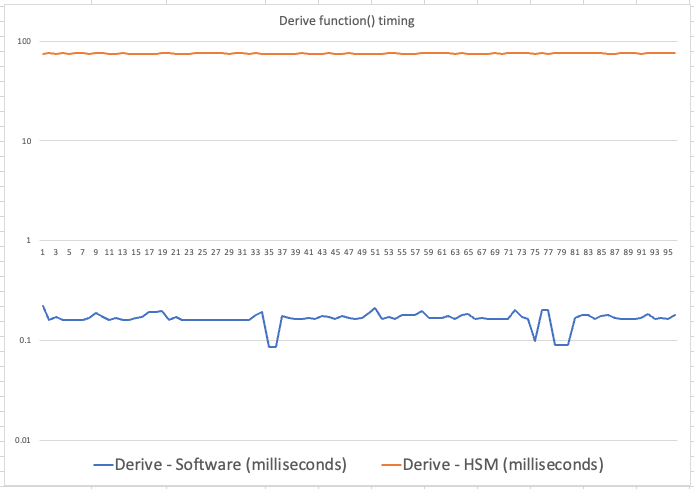
\includegraphics[width=1\linewidth]{paper/images/deriveFunctiongraph.png}
  \caption{Execution Time for DeriveNoise() and softwareDerive()}
  \label{fig:funcTimeGraph}
\end{minipage}%
\begin{minipage}{.5\textwidth}
  \centering
  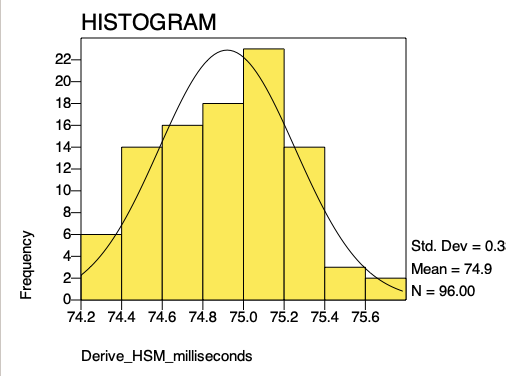
\includegraphics[width=1\linewidth]{paper/images/DeriveNoise freq.png}
  \caption{Histogram of DeriveNoise Execution Time in Milliseconds}
  \label{fig:hsmTimeGraph}
\end{minipage}
\end{figure}

The mean execution time for DeriveHSM() is 74.9 milliseconds and the standard deviation is 0.3 milliseconds. The variance across all data points is .11 milliseconds. 

The mean execution time for softwareDerive() is 0.17 milliseconds and the standard deviation is 0.02 milliseconds. The variance across all data points was too small to be significant.

\section{WireGuard-HSM lines of code}
The total number lines of code (LOC) changed in WireGuard-HSM when compared to WireGuard-Go are currently 104. If we subtract changes to the Read-me file and uapi.go file which handle configuration file changes and pkclient initialization, then the lines of code changed to the core WireGuard protocol files only amount to 44 LOC changes. A very easy number of changes to audit and understand.

\chapter {Discussion of Results}

Assessing the security of a new system is critical. A Deep knowledge of cryptography and mathematics are 

\subsection{security}
Our threat model assessment shows that WireGuard-HSM greatly improves the security of the WireGuard system by reducing the attack surface. Our system offers a higher level of security against zero days exploits by systematically separating sensitive data from the host system.

\subsection{performance}
The performance analysis shows the impact of using a USB-HSM in  WireGuard-HSM is less than a tenth of a second, so from a human user's perspective, this should be unnoticeable.
\section{portability}

A side-benefit of WireGuard-HSM's design is that the user's identify becomes physically portable because the private key is securely stored on a USB security key. When using WireGuard-HSM a user is able to securely carry their identify with them and use it on other machines running WireGuard-HSM.

\section {Limitations}
In this section I will discuss the limitations of my project in regards to the completeness of the evaluation and the limitations of the project implementation itself. Significant time was spent to get the technical implementation of the project working, so I will discuss what improvements I would like to see, if I had more time to complete the evaluation of the entire system.

\subsection{Formal Analysis}
A formal analysis was identified as an aspirational goal for this project. If I had more time, I would include a formal analysis of the security properties of WireGuard-HSM. The original WireGuard protocol has been verified using the Tamarin prover\cite{donenfeld_formal_2018}, so I would also like to define and verify WireGuard-HSM in the Tamarin prover to create a symbolic model of the system. This would further demonstrate how the security properties of WireGuard-HSM are correctly maintained.

\subsection{Mobile Operating Systems}
I had initially planned to support mobile operating systems such as a smart-phones. Users can easily use security keys
with mobile operating systems but due to technical requirements of the WireGuard protocol, a WireGuard-HSM user would have to leave their security key constantly connected
or after 2\textsuperscript{60} messages are exchanged. This could be avoided by having users modify their WireGuard client and peer defaults to a much longer timeout for re-key, but this seems like a burdensome approach and it may not be possible for the client to request a modification of peer settings.


\section{Compatibility}
WireGuard-HSM is able to perform a successful handshake and pass traffic with an unmodified WireGuard peer.

\chapter {Conclusion}
 
TODO !! In your conclusions section, you mostly focus on future work -- what are the actual conclusions you can draw from the results of your implementation, analysis, and experiments? !!

I have shown that WireGuard-HSM reduces the attack surface for threat actors by moving the long-term static private key into security key. WireGuard-HSM increases the portability of a user's identity while maintaining the security of the private key. This improves the ease-of-use for the user.

WireGuard-HSM increases the security by protecting the private key from threat actors.

WireGuard-HSM's performance impact was shown to be negligible, only adding about a tenth of a second to the handshake process.
WireGuard-HSM's user convenience impact was acceptable while adding physical portability to keys between machines,

\section {Future Work}
There are several areas where I would like to improve WireGuard-HSM that have been identified over the course of implementing and evaluating the system. These areas include pin handling and security key availability and kernel-mode support.

\subsection{Pin handling}
 A user may choose not a save the security-key pin in the WireGuard-HSM configuration file. In this mode, the program must prompt user for the pin. Currently this prompt is very simple and given on the command-line when the user runs WireGuard-HSM. This prompt is easy to miss and wouldn't work very well if WireGuard-HSM was implemented as a kernel module. A better approach would be to have the prompt implemented as a system-dialog window, that appears over any existing windows, making very simple for the user to omit the pin and only enter it when using WireGuard-HSM. Finding a Go-module that opens window dialogues and supports multiple operating system was deemed out of scope for this project but it will be my next addition to the program since it would increase the ease-of-use for the program. 
 
\subsection{Security Key Diversity}
Hardware security-key support for curve25519 and specifically X25519 is, as of writing, very limited. Nitrokey 3 is planned to support X25519 but the hardware is still not in mass production. I would like to see bio-metric hardware-keys with X25519 support, this would add an additional layer of security to our model as it further authenticates the user. As of writing, I could find no planned development for such a key. Many hardware-security keys have introduced support for near-field-communication (NFC) which makes using them with mobile devices almost seamless. Having a security-key with Curve25519 support, would make integrating WireGuard-HSM with mobiles devices easier and put less burden on the user. 

\subsection{Kernel-Mode Support}
WireGuard-HSM is written using the Go language version of WireGuard but a kernel-mode version would be more practical to most users. The Go-version of WireGuard warns users on start-up that if they are on a supported operating system, the kernel version has better support and offers better performance. The main challenge in writing the kernel mode version will be the PKCS\#11 integration and handling user interaction between a kernel module. A small program like pkclient that handled the PKCS\#11 integration and user prompts would be a good first step in expanding the functionality.

\subsection{Bio-metric Authentication}
It would be desirable for this project to use a bio-metric security key; for example, a security key that uses a small fingerprint reader to authenticate the user. A bio-metric security key with X25519 support is not yet offered together but they exist in independent implementations, for example Yubico sells a security key that has fingerprint reader needed for user authentication\cite{yubico_yubikey_2022}. 

\chapter{Recycling and Questions}
This will be removed in the final paper, just keeping items here for their reuse

\subsection{questions to answer}
Questions you need to be able to answer by your defense

    What is your contribution? What did you do that is worthy of being an MS Thesis/Capstone?

    What measurements are you taking? Part of your paper will be showing how "good" the system is. What are you using for comparison? How do you know that it is successful?

    What are the limitations? What could be done to improve those if you had more time? 
    What are alternatives decisions you could have made as you developed this and why didn't you choose those options? 
    We want to see that you thought through your work and that you made engineering decisions. 
        This is one of the points of receiving an MS degree is the implication that you have rigorous decision making process within the field of your expertise.
        
\section{Recycling}

\subsection {Conception}
I was interested in WireGuard when it was announced but it wasn't until a group project I started in Winter 2020, where we looked at the security of WireGuard and primarily identified key handling as a potential weak point in the program, that I began to consider different approaches to improving WireGuard,  without introducing a larger attack surface or forking the project. 

In Spring quarter of 2021, I took research methods in software development with Dr Erdly. During this course I continued to explore ideas that I had about WireGuard and its private key handling. I created my final project around WireGuard. In the project, I asked the question, how could WireGuard's private key handling be better? What systems could I create to improve it, and then how could I evaluate those systems?  
In the final part of the project I create a mock survey of software engineers to rate four of the final designs. I used my own metrics to define my terms (TODO finish up this back story, get to point about compatibility)

I came up with three designs that would improve key handling in WireGuard and I rated them on implementation, TODO(dig up project and look at ratings)!! In the end I chose the simplest overall design with the biggest risk being that my design relied on a security key produced by a single manufacture. No other manufacturer at the time sold a security key that supported X25519.

\subsection {Starting out}

I decided to start with interfacing with the NitroKey and getting familiar with the tools and commands to interact with it. I initially chose the Nitrokey start because the product page said it supported X25519\cite{noauthor_nitrokey_nodate} which is the ECDH key derivation process. After a few frustrating days I couldn't figure out how to even generate or put a curve25519 key on the nitrokey start. Searching online, I didn't see any existing software projects that interfaced with a security key for performing X25519 operations. What I did discover after pouring over NitroKey's documentation was that they recommended using a program called OpenSC to work with the Nitrokey but that only a program called GnuPG, when running in an advanced configuration mode, was capable of telling the Nitrokey to generate a set of curve25519 keys. Confusingly, GnuPG can generate the correct keys but it has no ability to perform X25519 with the security key.

\subsection {OpenSC}
Key derivation for ECDH, called X25519 in my specific case when using Curve25519 keys, requires access to Bob's private key and Alice's public key. The cryptographic operation will generate a new 'shared key' that is identical for both parties when the keys are flipped and you use Alice's private key and Bob's public key. 
After researching the OpenSC tool support forums, I was able to find the command string that instructs a  security key to perform the key derivation operation with the correct inputs and outputs. However the tool only produced an error when I tried to use it with the Nitrokey and Alice's public key. I discovered that while NitroKey support documentation says OpenSC is the best tool to use with a Nitrokey Start, OpenSC doesn't support reading curve25519 keys! Why would this key list support for X25519 then? I found out that there was a single test that was written in OpenSC which used the PKCS\#11 interface to generate and verify a shared-secret on the hardware device. This functionality wasn't exposed to users in any way and only ran as part of a test-suite for part of the program. Technically, OpenSC could be used to test that X25519 operations worked on a hardware device but with no user control over the process. This realization set the stage for the rest of the project: technically the functionality is there but no-one has a practical implementation yet. I enjoy a challenge but I was getting worried at this point about the feasibility of completing my project on time.

At this point, I realized that had I created a proof-of-concept program before starting my project, it would have been helpful in gauging how much work this project would entail. It was a frustrating start to my project, I couldn't even start on modifying WireGuard to use the NitroKey if I couldn't find a way to perform X25519.

Analysing the key derivation function in OpenSC and finding the spot where reading my key failed, gave me enough information to start looking into how OpenSC read keys using OpenSSL and then I researched Curve25519 support in OpenSSL. Curve25519 support was a relatively recent addition in version 1.1 of the program\cite{noauthor_support_nodate}.
After digging through the OpenSC tool some more and reading the OpenSSL function documentation, I was able to upgrade how OpenSC read public keys during key derivation and expand its functionality to support X25519 and get the previous command working.
Once I had OpenSC working to perform X25519 on the key, I wrote a test that would perform the operation on the security key and also perform the operation as the other party but in software-only mode, using OpenSSL. The test would verify that the derived key was the same from both steps of the test. This test confirmed that the security key's X25519 function worked correctly and I was finally making progress.

At this point, I realized that all of OpenSC's interaction with the security key is handled via the PKCS\#11 interface and that interface is compiled into a library which connects to the operating system. This library abstracts parts of the lower-level system interactions, so I wouldn't need to worry about, for example, the USB interface. I spent some time looking at how other programs use PKCS\#11 libraries to implement hardware key integration to get more familiar with this area of programming.

\subsection{Interfacing}
At this stage I had X25519 working on the security key and I understood more about PKCS\#11 and how other programs used it. This interfacing part was the area of my proposal that I understood the least. Before I started the project, I wasn't that clear about exactly how I would 'connect' X25519 operations and WireGuard. Using my software development skills that I learned at the UW, I decided it would be best to encapsulate the functionality in a program that would act as the go-between. Handing the various states of the program, user-input and error states. I could create my own limited API for a calling program to request specific actions on the security key. This approach would also reduce the amount of work I would have to do in WireGuard itself.

\subsection{WireGuard Implementation Choice}
I had assumed at the beginning of the project that I should implement my program by modifying the Linux kernel module version of WireGuard. I tried for a few days to learn how to modify and build a kernel module, which has gotten a lot more complicated and time-consuming with things such as module signing and the sheer size of the Linux kernel. I had written and built a kernel module in CSS 537 but that module didn't need to interact with external libraries or handle bi-directional user interactions. After reading the WireGuard kernel module, I decided to try reading through the Go language version of WireGuard. This version is implemented as a standalone program that can run on most operating systems. This version was easier to comprehend and understand the program flow. My project is about implementing new functionality and evaluating the system, so I decided to focus my efforts into modifying the Go version of WireGuard.
The Go programming language has good support for modules which allows programs to easily expand their functionality by importing other code modules. After some more research, I decided to create a Golang module that handled the physical security-key interface and expose a restricted set of functionality to a calling program. 

\section{Configuration}
WireGuard configuration on the command-line is handled via a separate program called wireguard-tools \cite{noauthor_wireguard-tools_2022}. This program handles parsing a plain-text configuration file and turns the configuration directives into API calls to the separately running WireGuard daemon, which configures the virtual-interface. I wanted my program to conform as closely as possible to the WireGuard reference implementation, so I made modifications to the wireguard-tools program. I added support for an 'HSM' line in the plain-text configuration file. 

This modification removes the requirement for defining and storing the private-key in the plain-text file. The HSM directive tells the program two, and optionally three things. First it lists the PKCS\#11 library path. Second, the slot id  to use on the security key. Thirdly and optionally, the pin required to access the slot.

The detailed workings of the PKCS\#11 interface are out of scope for this paper, however it suffices to say that for interfacing with a security-key, PKCS\#11 requires a slot ID and a secret pin-number for that slot to enable privileged operations such as key-signing or key derivation. The PKCS\#11 interface will inform the caller if they successfully logged into the slot and if the requested operation succeeded or not.

Security is a balancing act between overall system security and user-convenience. Making a system more secure can often come at expense of user-convenience. 

(TODO merge into section above
In the WireGuard protocol, both parties are identified by their static public key.  The most important fields in the handshake message are shown in Figure \ref{fig:hand_init}.

To create an initiation message, the initiator generates an ephemeral, Curve25519 key-pair. The ephemeral public key is added to the message. The initiator's static public key is encrypted using ChaCha20Poly1350 AEAD. The encryption key for this field is a derived key, which is derived in-part using the responders static public key.
The sender's index is a randomly generated 4-byte value. It is used as a peer's chosen handshake session id.
The responder's public key used as key to MAC 1. This initiation message contains an encrypted form of the initiator's public key.

The contents of the initiation message are authenticated using MAC 1.
A MAC is used to protect the initiation message, with the MAC key being the responders public key.

responder, an initiator is identified by their ability to decrypt messages encrypted with the client's public key, and cannot be revoked, except by manually notifying and removing the client’s public key from all servers. As mentioned previously, in WireGuard, key management is intentionally left up to the users and administrators. There is no certificate revocation mechanism or expiration of client and server keys.

MAC2 is an optional message authentication code and is only used when the anti-DDoS mechanism is enabled for a given responder. While this feature is interesting from the protocol security perspective, further discussion of these features is out of scope for the project.

A strength of the pre-shared static public key requirement, is that any party running WireGuard is resistant to active network enumeration. In order to elicit a response from a node running WireGuard, the initiator's message must have knowledge of the responder's public key, in order to properly form the handshake initiation packet.
)
===================================

\subsection{Threat Modeling System state assumptions}
Assumptions about program and system state. When considering diagramming and system, we need to make several assumptions about the system state. That is, What doe the use case look like? How are the users interacting with the system? What mistakes could the user make when using this system? Does the model we are using capture all of them?
I want to draw attention to key designs about the system and its basic parts related to private key handling.
Alice inserts in the hardware security key when she intends to use WireGuard to connect to Bob. Alice enters her security key pin every time when using it. 


\bibliographystyle{plain}
\bibliography{references}
\end{document}
